\documentclass{beamer}

% for themes, etc.
\mode<presentation>
{ \usetheme{metropolis} }
%{ \usetheme{boxes} }

\usepackage{times}  % fonts are up to you
\usepackage{graphicx}

% these will be used later in the title page
\title{South Africa ALICE Computing}
\author{Sean Murray \& William Phukungoane\\
    CHPC,CSIR \\
    University of Cape Town 
}

\date{April 17 2017}

% note: do NOT include a \maketitle line; also note that this title
% material goes BEFORE the \begin{document}

% have this if you'd like a recurring outline
\AtBeginSection[]  % "Beamer, do the following at the start of every section"
{
\begin{frame}%<beamer> 
\frametitle{Outline} % make a frame titled "Outline"
\tableofcontents[currentsection]  % show TOC and highlight current section
\end{frame}
}

\begin{document}

% this prints title, author etc. info from above
\begin{frame}
\titlepage
%but first the important stuff.
\end{frame}

\section{Current Status (last year)}
\begin{frame}
    \frametitle{Location}
    \centering{
    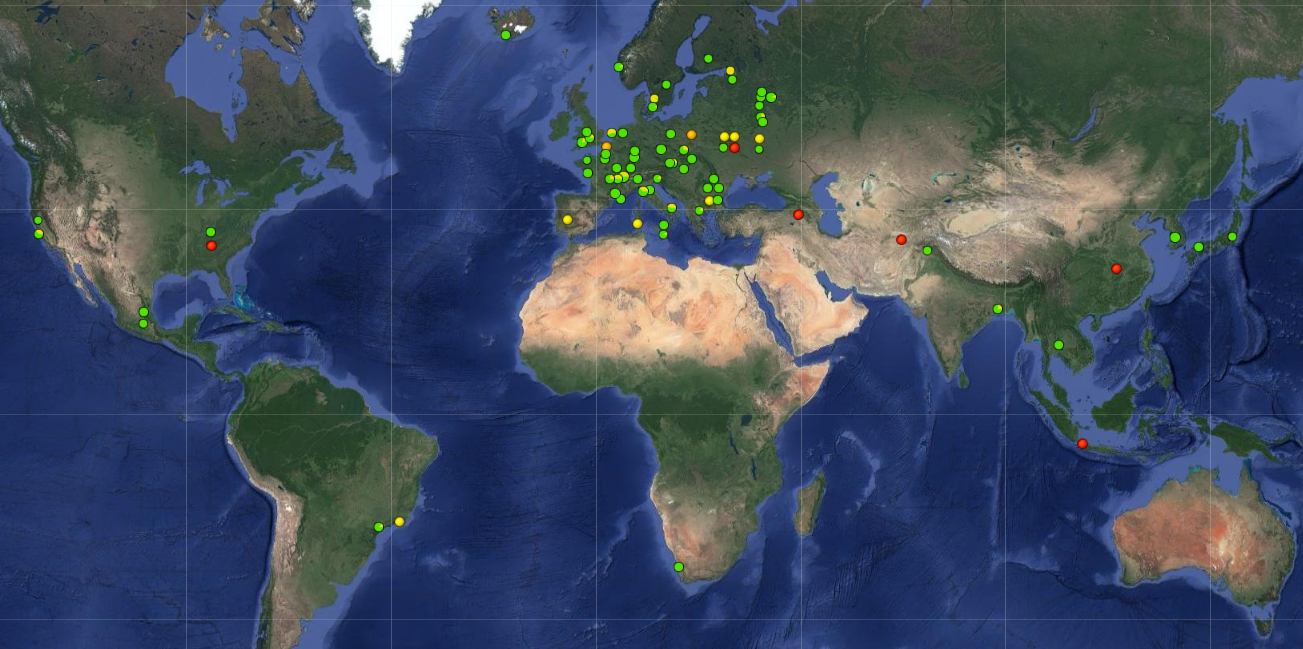
\includegraphics[scale=0.35]{ALICEGridSites.png}
}
\end{frame}
\begin{frame}
    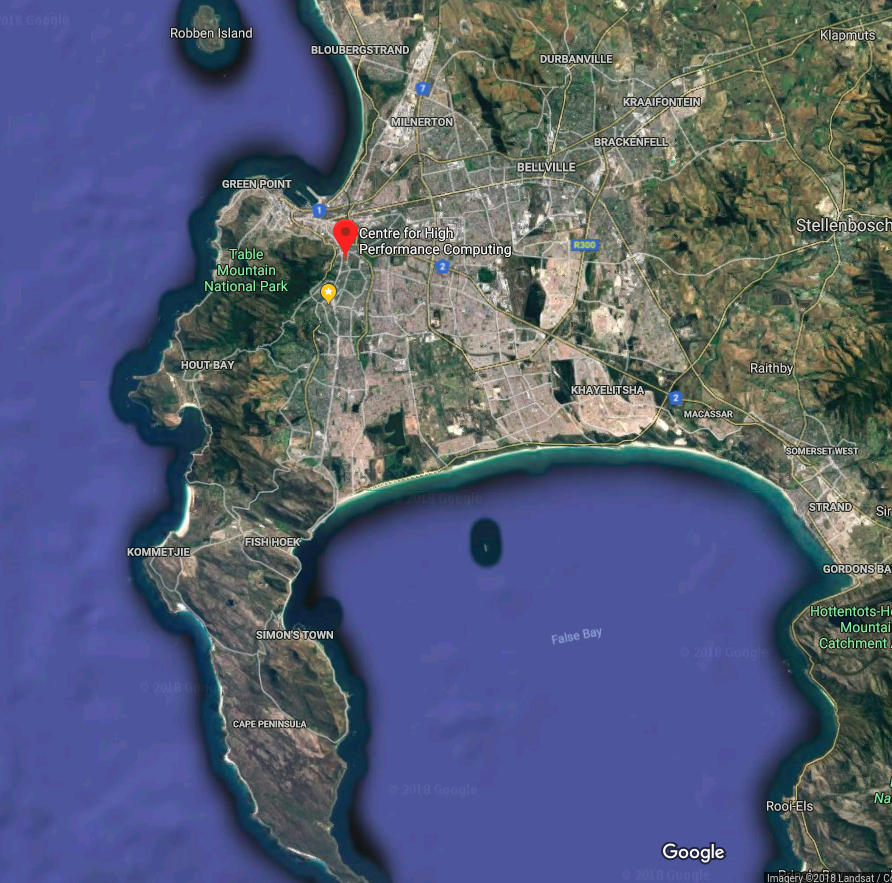
\includegraphics[scale=0.5]{CPTmap.png}
\end{frame}


\begin{frame}
\frametitle{Commitments}
Resources Delivered and pledged.
    \begin{tabular}{|r|r|r|r|r|r|}
        expriment&  index     & 2017  & 2017  & 2018   & 2018    \\ \hline
        ALICE         & cpu  & 12000  & 6000 & 10000  & 10000   \\ \hline
                 & disk & 348TB & 100TB & 1500TB & 1500TB \\ \hline
        ATLAS        & cpu  & 12000  & 0 & 10000  & 10000   \\ \hline
                 & disk & 262T0B & 0TB & 700TB & 700TB \\ \hline
    \end{tabular}
\end{frame}

\begin{frame}
  \frametitle{Computing Infrastructure}
  \centering{
  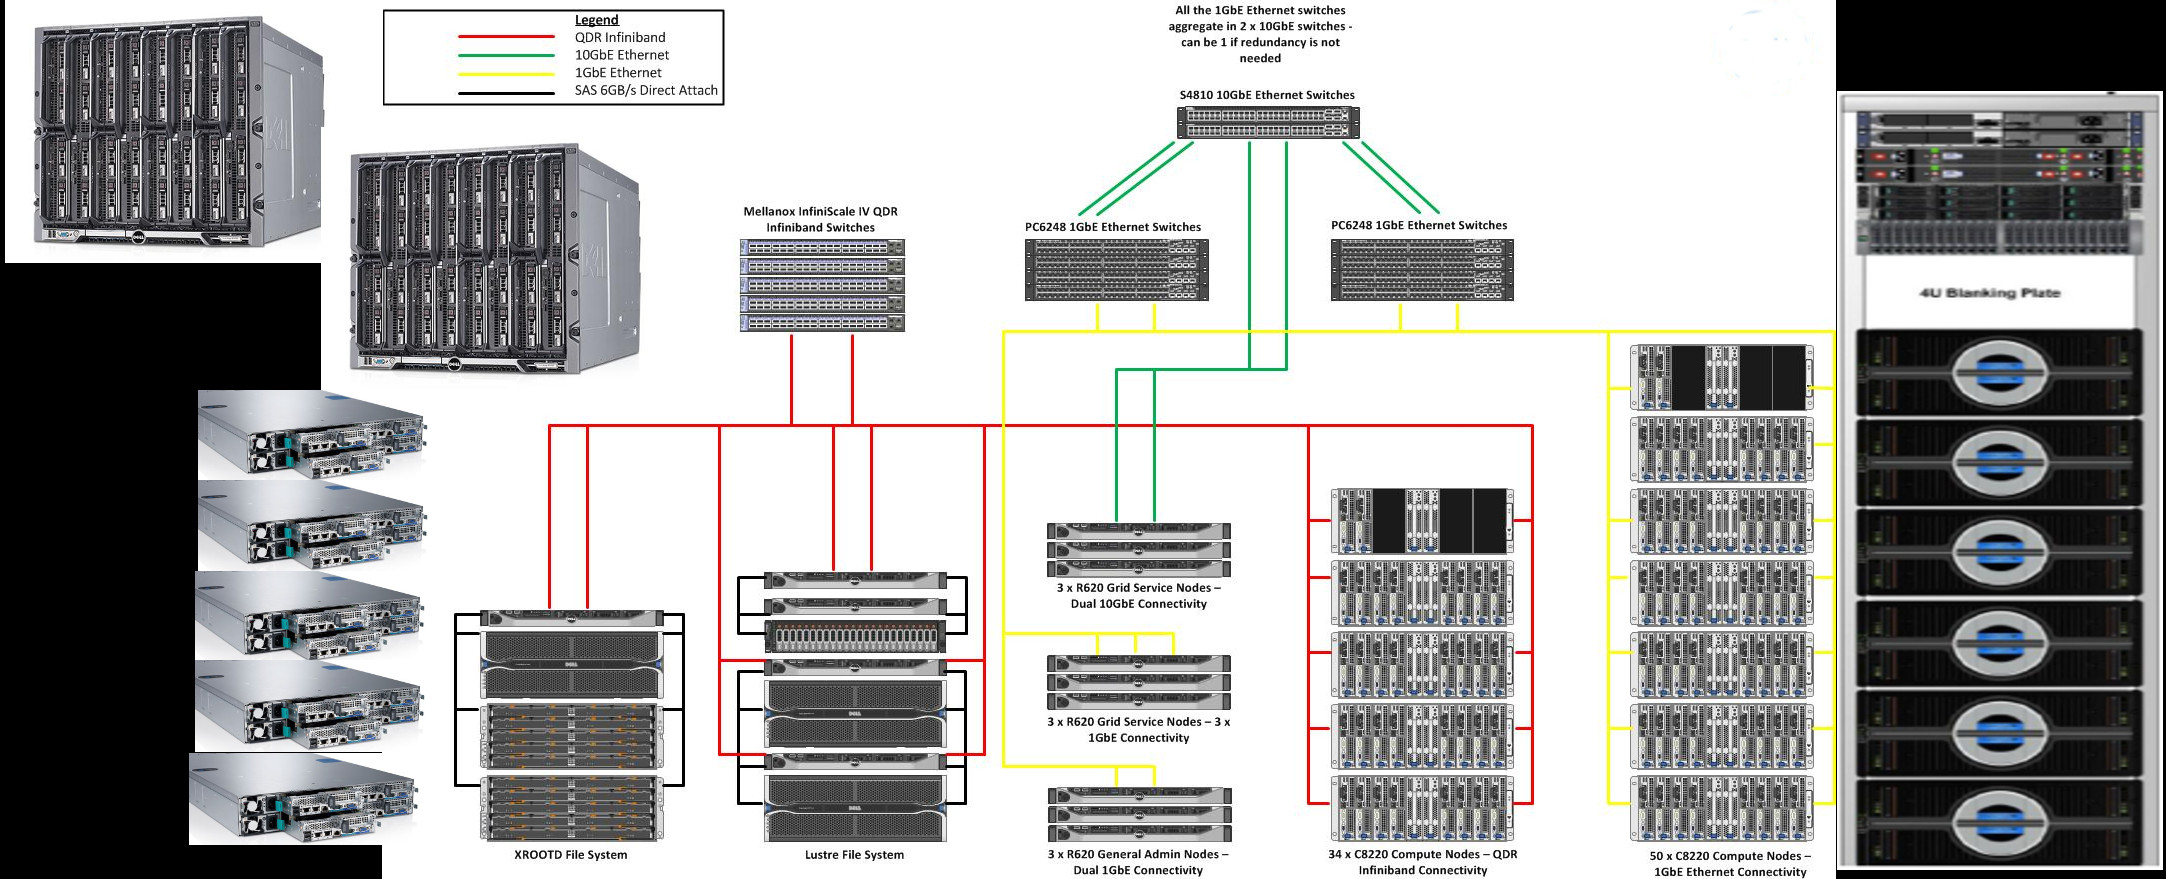
\includegraphics[scale=0.2]{CHPCConnectivityDiagram.jpg}
  }
\end{frame}

\begin{frame}
  \frametitle{Current hardware}
  \begin{itemize}
    \item 50 nodes of 48 cores 192GB RAM and 1.6TB of SSD, 2x bonded 1G ethernet
    \item 29 nodes of 48 cores 96GB RAM and 1TB, QDR infiniband.
    \item 2x M1000E (16 blades) "new"
    \item 5xC6100 8x 6core xeon each. "new" 
    \item 9 management servers, lower spec
  \begin{itemize}
    \item compute element (head node,ce),
    \item storage element 2 redirectors, 2 storage nodes with direct attached multipath storage
    \item authentication, monitoring, provisioning. 
  \end{itemize}
  \end{itemize}
%TODO NO maintenance contract
\end{frame}

\begin{frame}
  \frametitle{Current Storage}
  \begin{itemize}
    \item 383TB EOS for ALICE
    \item 252TB EOS for ATLAS
    \item 1PB Lustre via QDR infiniband, no ups and Xyratex proprietary hardware.
  \end{itemize}
    Storage is limited to c. 4Gbps which limits processing hence not all cores are allocated.
\end{frame}

\begin{frame}
  \frametitle{Current Performance last year}
    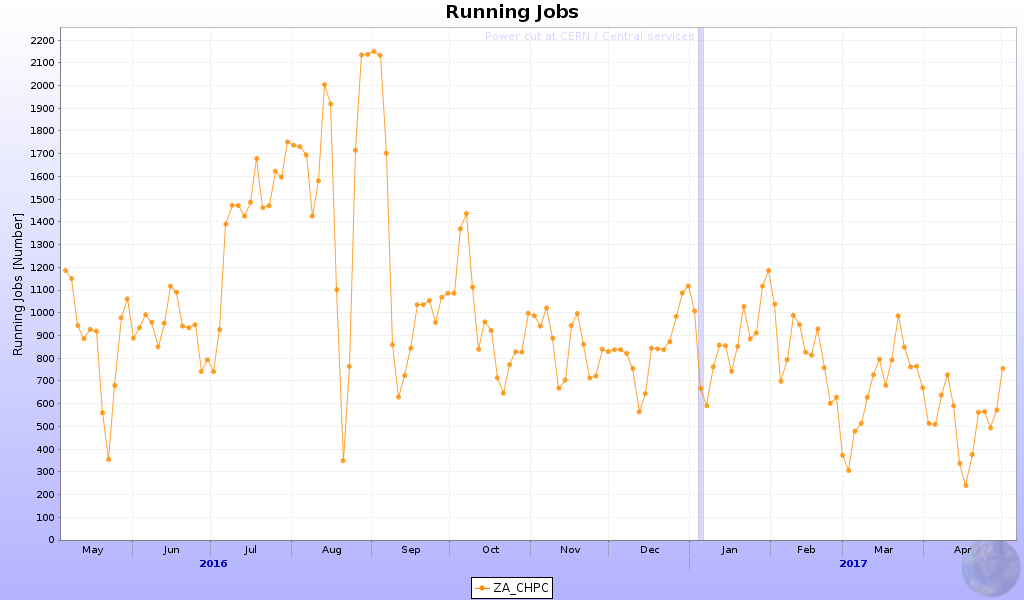
\includegraphics[scale=0.25]{ALICERunning1Year.png}
\begin{itemize}%TODO with a graph
  \item 1.7M ALICE jobs in last year, 877k 2016, 455k 2015.
  \item 1222 Avg 2017  980 Avg 2016 704 Avg 2015.
  \item 293TB of 383TB, 91TB last year. Dec 15-Jan 29 we took in 100TB, 30\% of our storage, mostly CERN and FZK
\end{itemize}
\end{frame}

\begin{frame}
    \frametitle{Graph of Storage Use}
    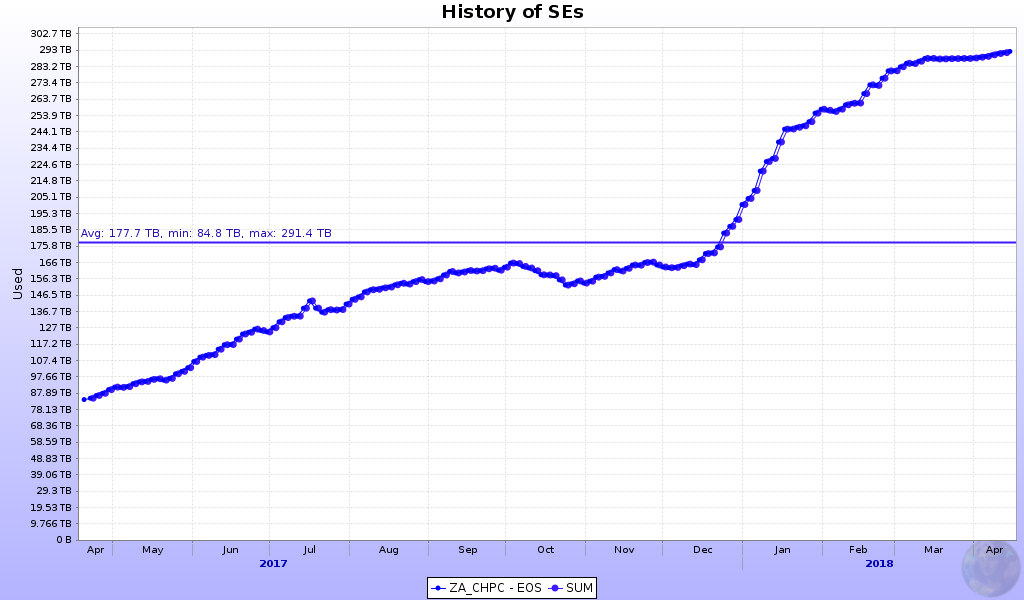
\includegraphics[scale=0.25]{ALICEStorageUtilisation.png}
\end{frame}

\begin{frame}
    \frametitle{Graph of Storage Transfers}
    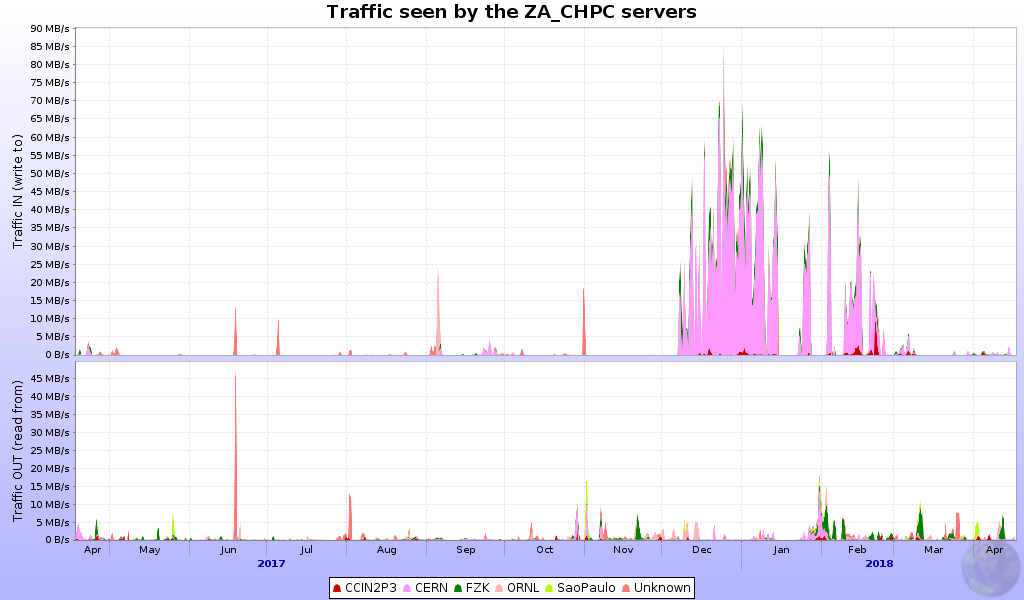
\includegraphics[scale=0.25]{StorageTrafficInandOut.png}
    100TB from 15 December to 29 January.
\end{frame}
\begin{frame}
  \frametitle{Availability / Reliability}
    \centering{
    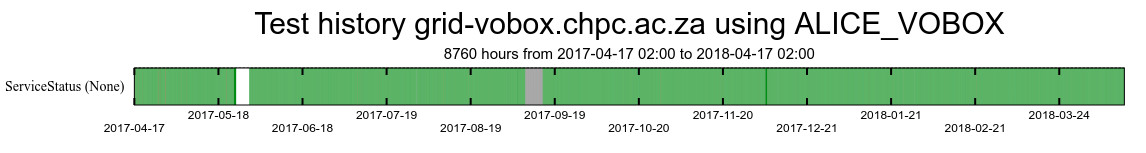
\includegraphics[scale=0.35]{SAMS-VOBOX.jpg}\\
    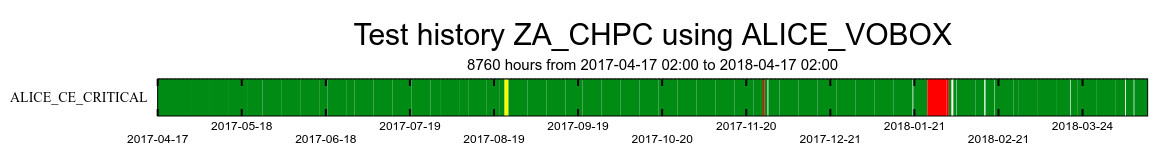
\includegraphics[scale=0.35]{SAMS-CE.jpg}
}
    \newline
    \centering{
\begin{tabular}{|c|r|}
  Function     &  Last 365 days \\ \hline 
  Availability &  96\%  \\ \hline
  Reliability  &  95\%  \\ \hline
  Storage & 72\% \\ \hline
\end{tabular}
}\\
\vspace{0.5cm}
\end{frame}
\begin{frame}
    \frametitle{EOS "downtime"}
    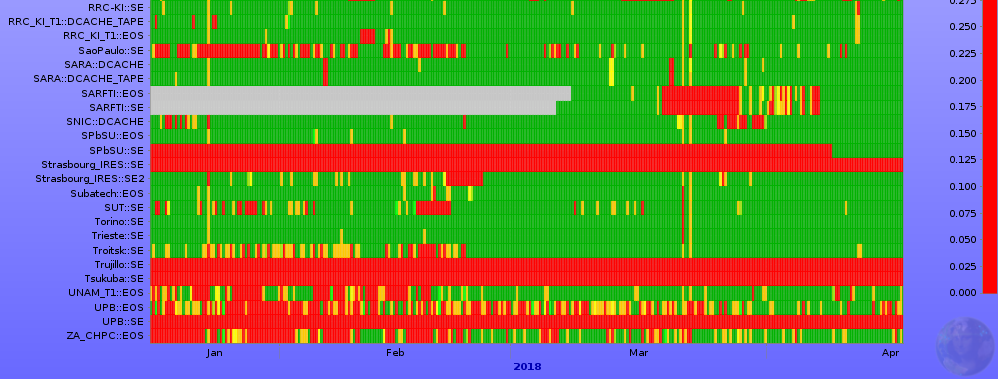
\includegraphics[scale=0.25]{EOS-Status-3monthsa.png} \\
Storage down time is primarily due to storage test failures due to network starvation. Its now gotten so bad it happens 7 or 8 times a week.
\end{frame}
\begin{frame}
\frametitle{Downtimes}
The big ones are, ignoring network starvation :
\begin{itemize}
    \item 25 January Failure 1.5 week, to get new certificates.
  \item 27 Nov Melted busbar, we managed to patch power across and keep system up, while power was switched off and redone.
\end{itemize}
\end{frame}

\begin{frame}
    \frametitle{Network maximisation}
    We have maxed out our network at 2.1Gbps regularly.
    \begin{itemize}
            \item CE at 1Gbps
                \item EOS at 1Gbps
                \item Vobox doing a 100Mbps.
    \end{itemize}
\end{frame} 

\begin{frame}
    \frametitle{provided and (required)}
\vspace{0.5cm}
\centering{
\begin{tabular}{|c|c|c|c|c|}
    Resource          &  2016          & 2017              & 2018         & 2019 \\ \hline 
    CPU     kHS06     &  7.5 (6)       & 7.5 (7.5)         & 10(8.09)    & 15(12.35)  \\ \hline
    Storage    TB     &  384 (550)     &  384 (682)  & 15000(1100)   & ??  \\ \hline
\end{tabular}
}
\end{frame}

\begin{frame}
    \frametitle{Cpu graphically hepspec06-10}
    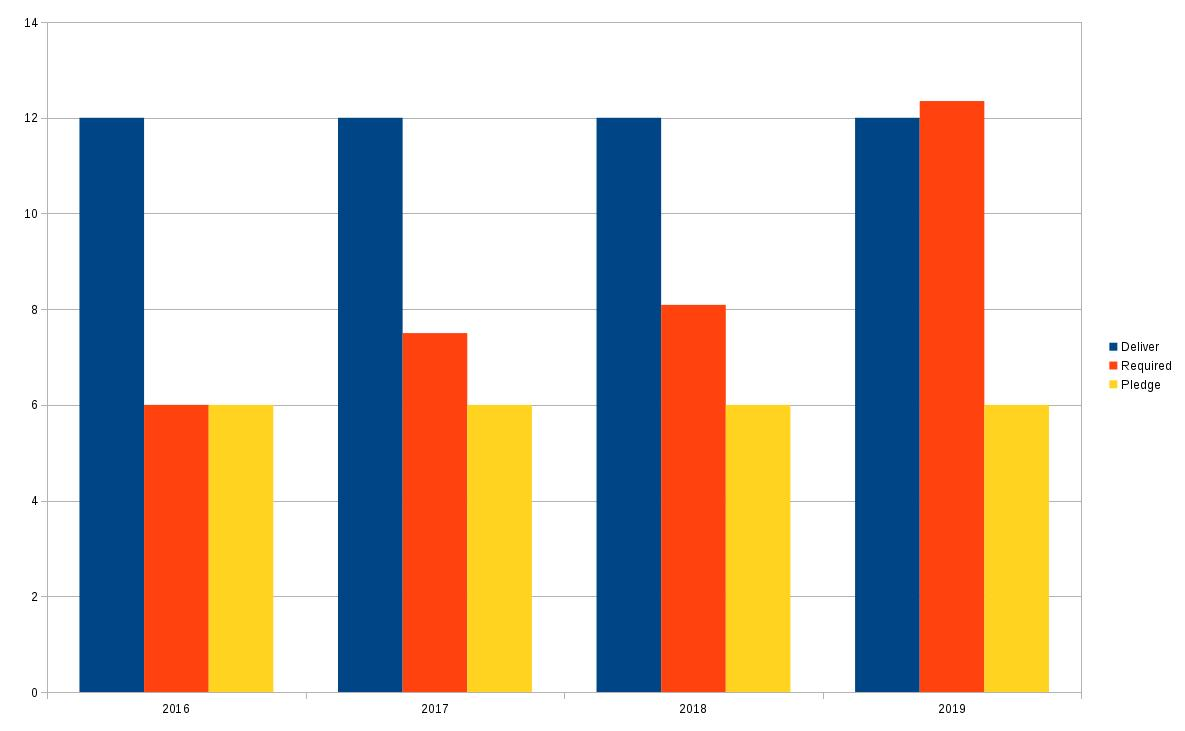
\includegraphics[scale=0.35]{CPUPledge-10.jpg}
\end{frame}

\section{Going Forward}
\subsection{CPU}
\begin{frame}
    \frametitle{cpu growth}
    \begin{itemize}
    \item No real plans here(money), migrate computing into the lower spec 29 nodes
    \item Project for openstack cloud onsite.
        \item We picked up 2 M1000e blade systems and 5 dell c6100.
    \item openshift on our M1000e and C6100 cpu additions. Build farm, testing, and batch when idle.
    \item We could allocate 3400 cores, hepscp06=12.
    \end{itemize}

\end{frame}


\subsection{Storage}
\begin{frame}
    \frametitle{Storage}
    \begin{itemize}
            \item<1-> After much frustation with the 100TB of Lustre it will become central storage for openshift
            \item<2-> We have 1PB of lustre, connected to 29 grid nodes and 1 M1000e via QDR.
            \item<3-> we were allocated 2M ZAR, to meet pledges of storage, 1.5PB ALICE.
            \item<4-> Addtional 2.4M ZAR found from excess budgets from SA-CERN collaboration excess funding.
            \item<5-> In Total 4.4M ZAR (280k EUR) for new EOS Storage, strings attached.
            \item<6-> Attempts to make EOS generic off lustre storage for site.
    \end{itemize}
    \end{frame}
\subsection{Network}

\begin{frame}
  \frametitle{Network Connection}
  \centering{
  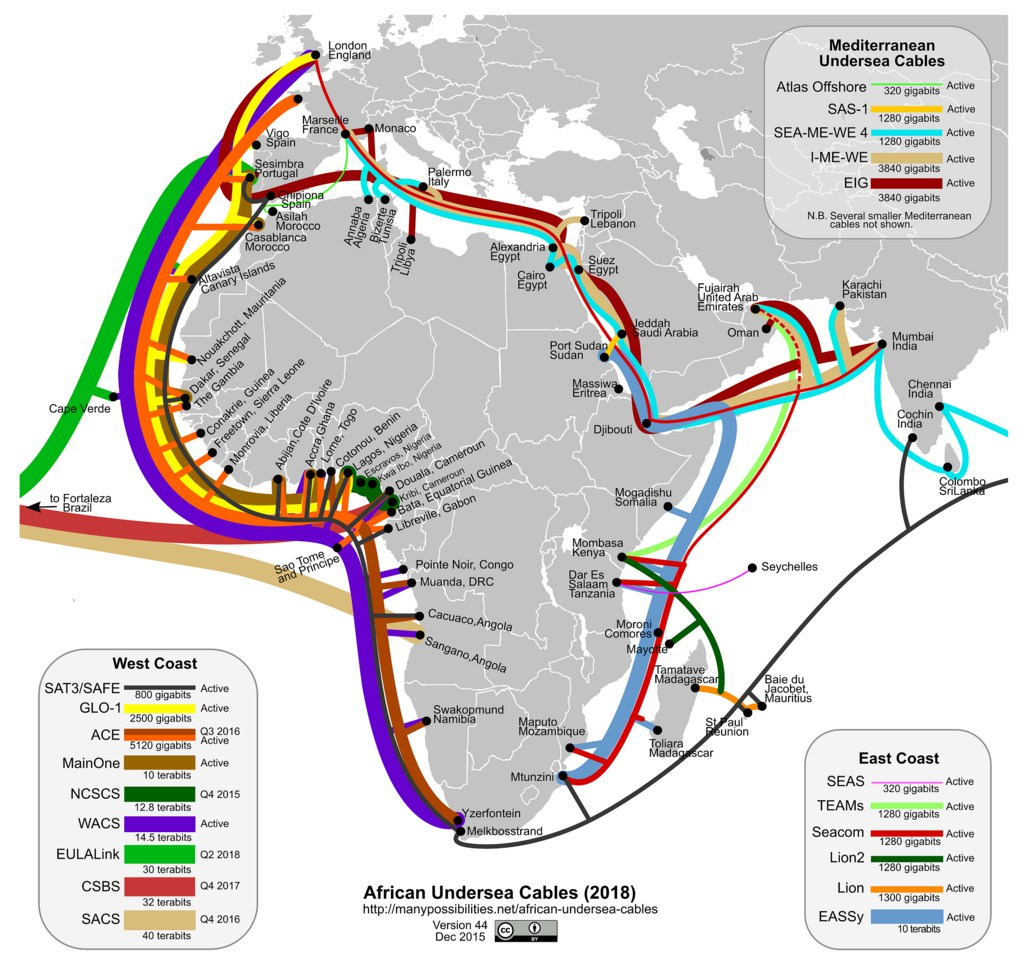
\includegraphics[scale=1]{african_undersea_cables.jpg}

We are now connected directly to the SANREN backbone at 10Gbps.}
\end{frame}

\begin{frame}
    \begin{itemize}
            \item 10G network installed
        \item new ipv4 and ipv6 allocated.
        \item  Tested on 1 node on ipv4 and ipv6.
                \item still waiting for sfp purchase, currently using a donation.
                    \item We are on the backbone, naked.
                        \item We are still only paying for 212Mbps.
    \end{itemize}
\end{frame}


\section{Alternate users, the cpu slush fund.}

\begin{frame}
\frametitle{29 nodes} %TODO explain 28 nodes, M1000e's code-rade building and spare resources.
\begin{itemize}
  \item 29 nodes local HEP, and grid, and generic usage.
  \item M1000e and C6100 for slush fund addition. (donations)
  \item code based on CODE-RADE, or LHC experiments from CVMFS.
  \item Local Storage for users, eos and beegfs.
\end{itemize}
The idea was to run the 29 nodes, 1392 cores with 1PB beegfs as a proof of concept of a analysis facility rather than a Tier1. 
\end{frame}

\section{Ecosystems}
\begin{frame}
    \frametitle{Square Kilometer Array}
    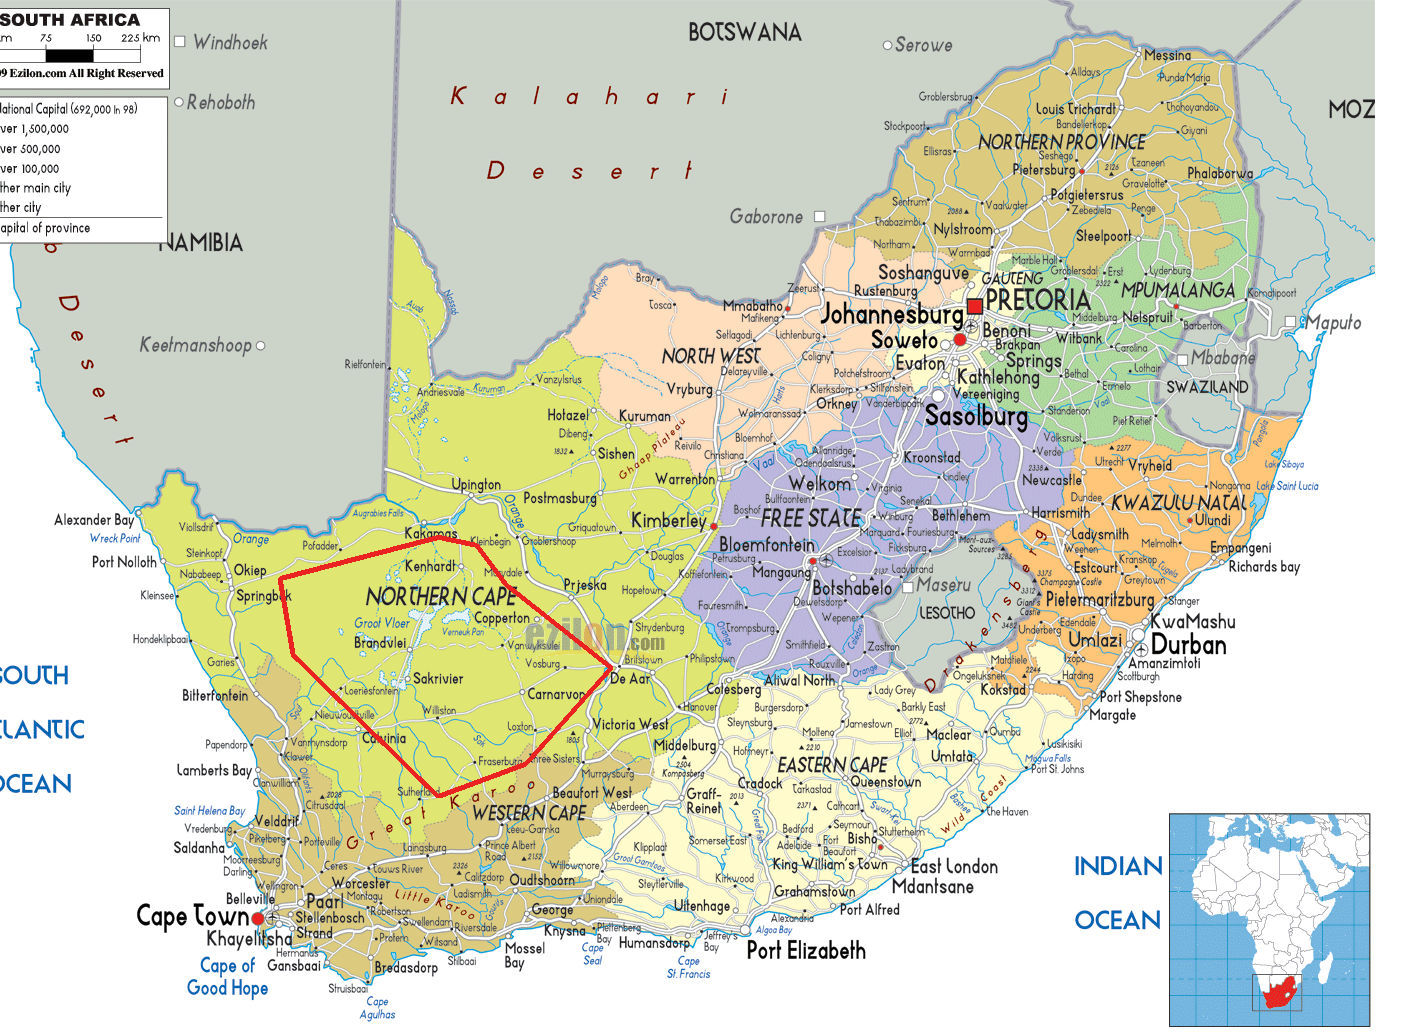
\includegraphics[scale=0.25]{ska-radiosilence.png}
\end{frame}

\begin{frame}
    \frametitle{Square Kilometer Array, partners}
    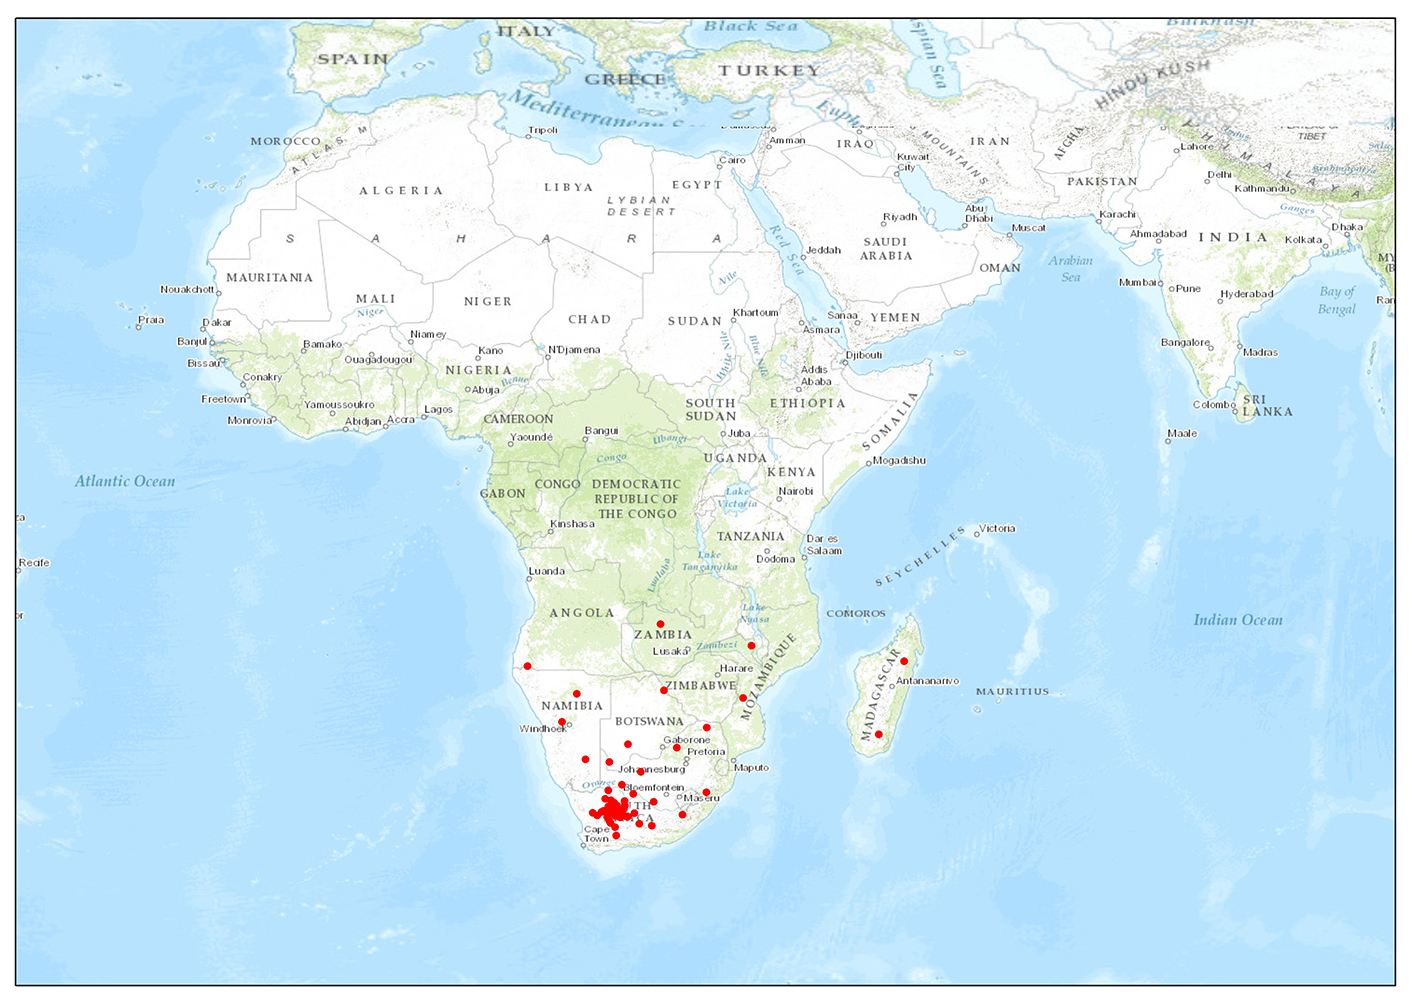
\includegraphics[scale=0.25]{ska_partners.jpg}
\end{frame}
\begin{frame}
    \frametitle{Stampede} %TODO explain ecosystems somehow.
    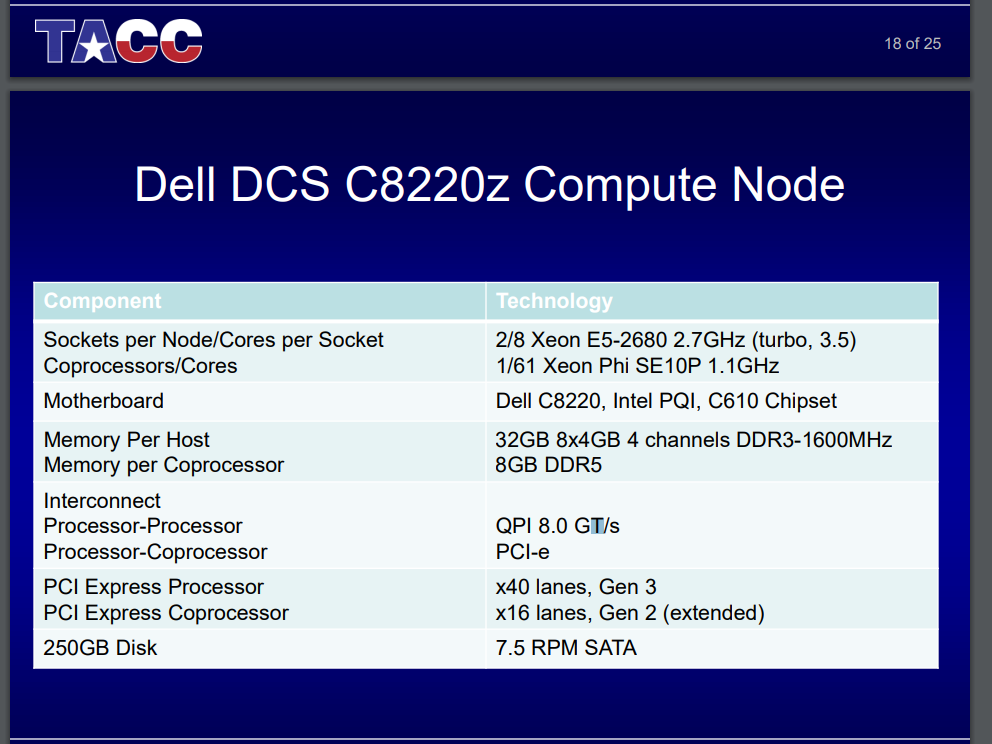
\includegraphics[scale=0.25]{tacc_stampede.png}
    20 racks currently mid-Atlantic.
\end{frame}
\begin{frame}
    \frametitle{Mozambique President}
    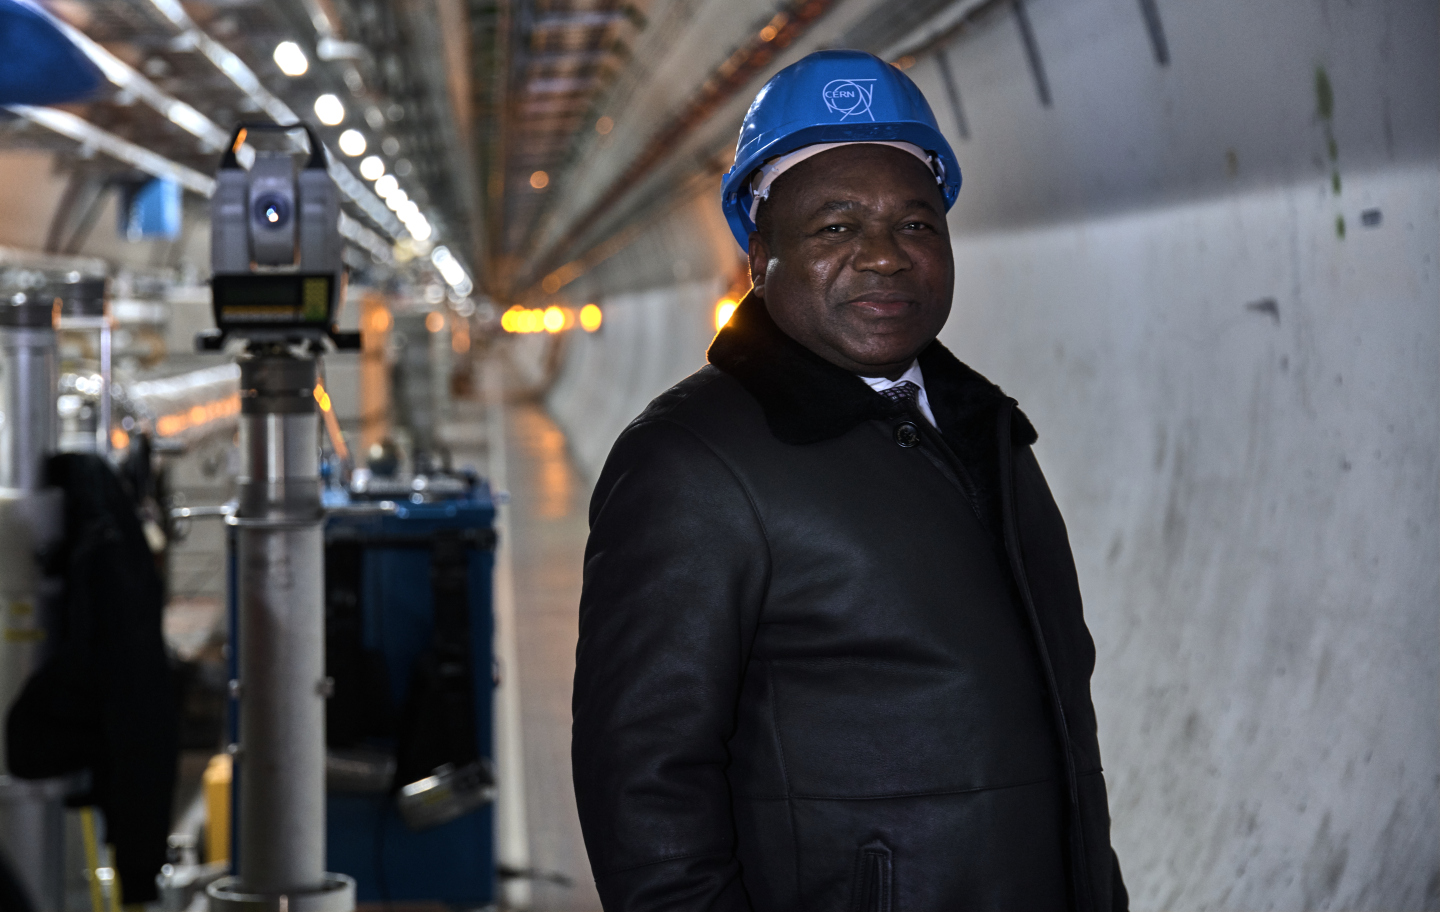
\includegraphics[scale=1]{Moz-Pres.jpg}
\end{frame}
\begin{frame}
    \frametitle{Mozambique}
    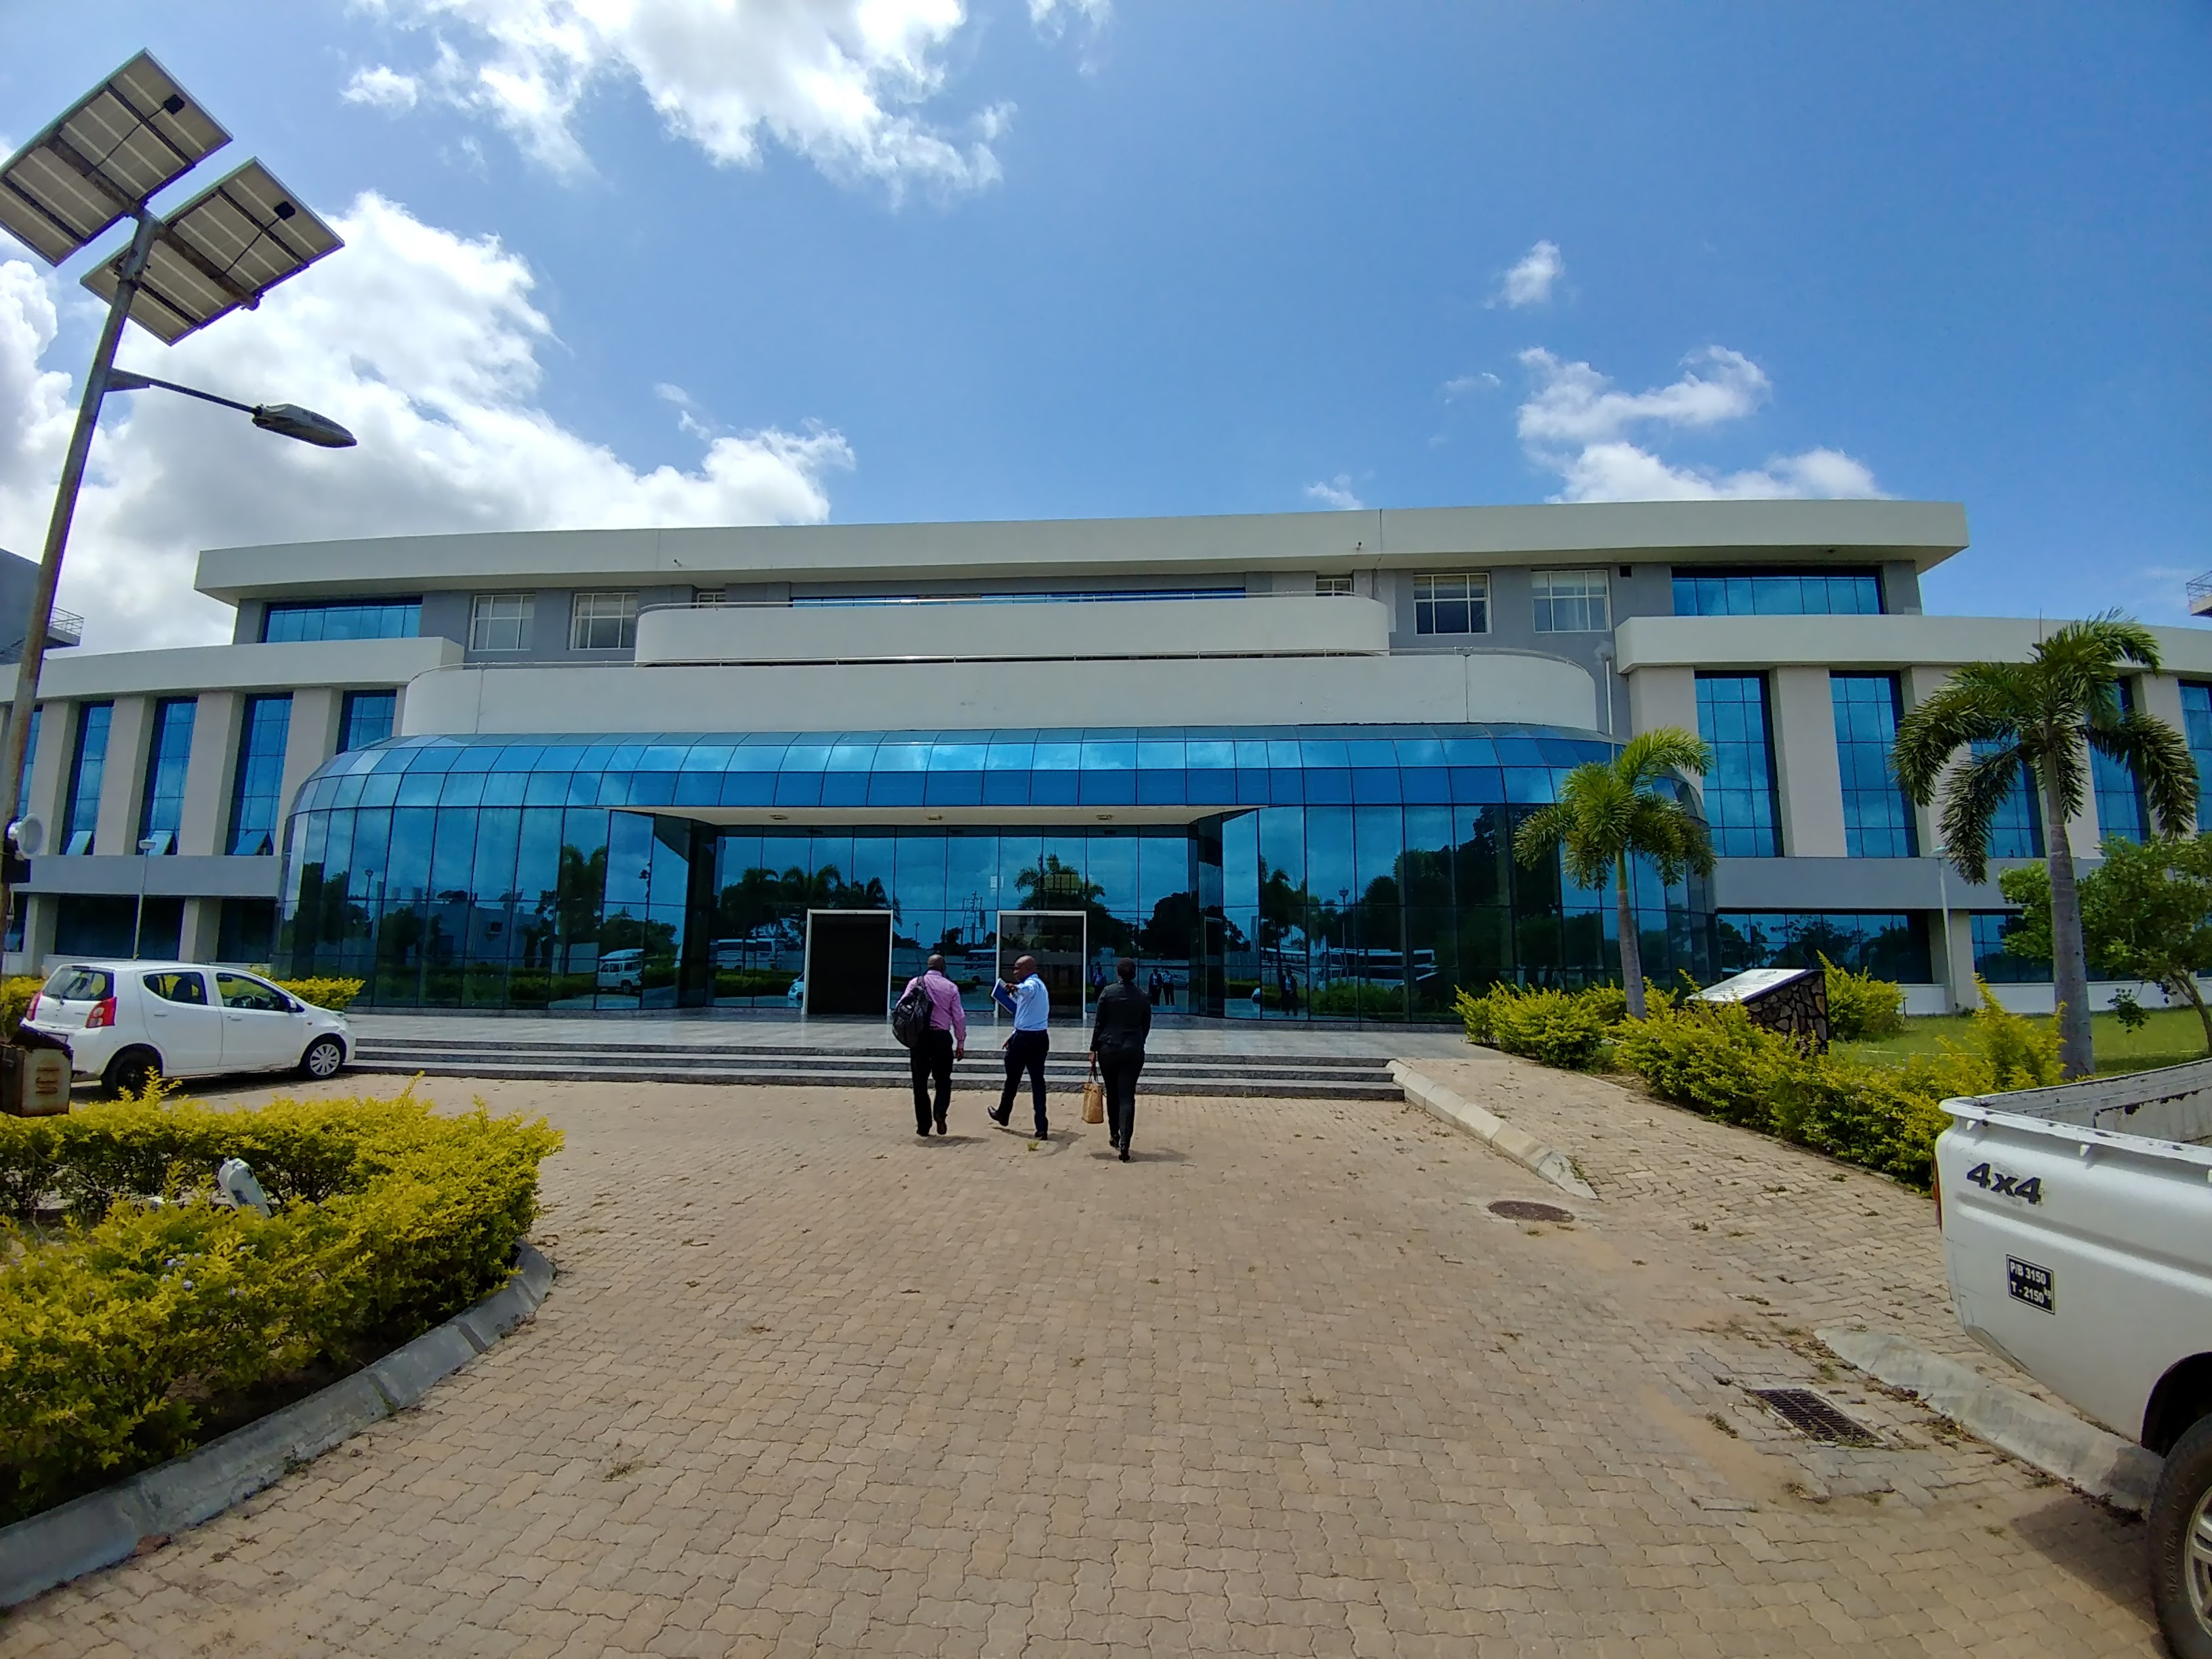
\includegraphics[scale=0.1]{MozambiqueDataCentre.jpg}
    Space for 80 racks, brand new.
\end{frame}
\begin{frame}
    \frametitle{Mauritius}
    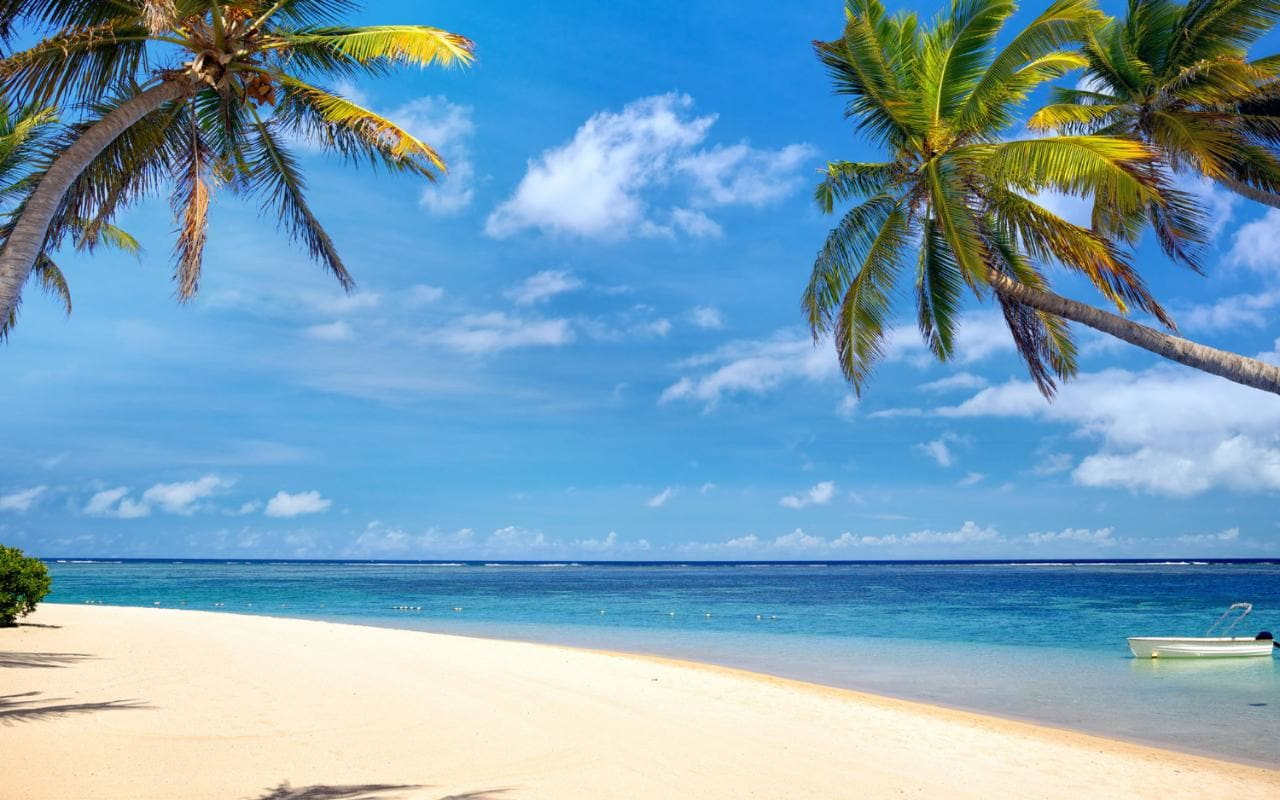
\includegraphics[scale=0.25]{Mauritius-Beaches-Tropical-beach-xlarge.jpg}
\end{frame}
\begin{frame}
    \frametitle{Mauritius}
    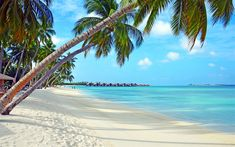
\includegraphics[scale=1.5]{Mauritius-Beaches2.jpg}
\end{frame}
\begin{frame}
    \frametitle{Mauritius}
    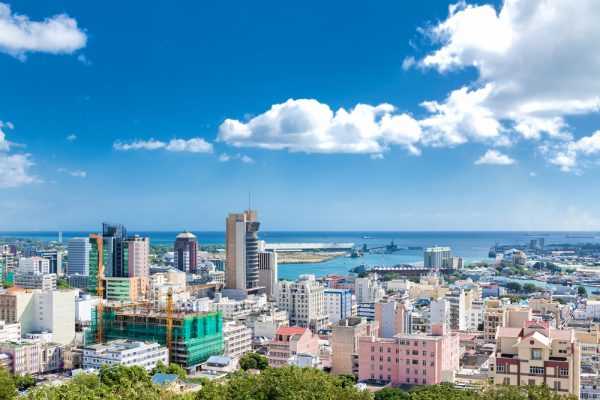
\includegraphics[scale=0.5]{MauritiusCBD.jpg}
\end{frame}
\section{Summary}

\begin{frame}
    \frametitle{Summary}
    Things are improving.
    \begin{itemize}
        \item The big impediment of network is now a purely technical config issue, and money, we are using a donated network at the moment.
        \item Storage is shortly to exceed the required amount for the first time.
        \item Ample cpu.
    \end{itemize}
\end{frame}


\end{document}
